\chapter{Design Flow}
\label{sec:design-flow}

In this chapter we introduce a novel design flow for creating
high-performance dataflow designs starting from C/C++ applications. We
explain the motivation and requirements for the proposed approach and
provide an overview of the three main components: the \FAST{}
language, the Aspect repository and weaver and the compilation
backend. We show how these three components can be integrated to
produce an automated design technique. We analyse the steps required
to produce an optimised design using the proposed approach and compare
this with alternative approaches using other start-of-the-art
technologies. Finally, we present an extension to our original
design-flow to support run-time reconfiguration.


\section{Overview}

Figure \ref{fig:design-flow-overview} provides a brief overview of the
proposed design flow. First a high level application is produced as
the input to our flow. This is then partitioned into a software part
and a hardware part to run on the dataflow accelerator. A dataflow
kernel is generated from the original description. Aspect descriptions
are used to control the optimisation process.

Thus the inputs to the design flow are:
\begin{itemize}
\item High-level source specification
\item Aspect descriptions for controlling the compilation process
\end{itemize}

\begin{figure}[!h]
  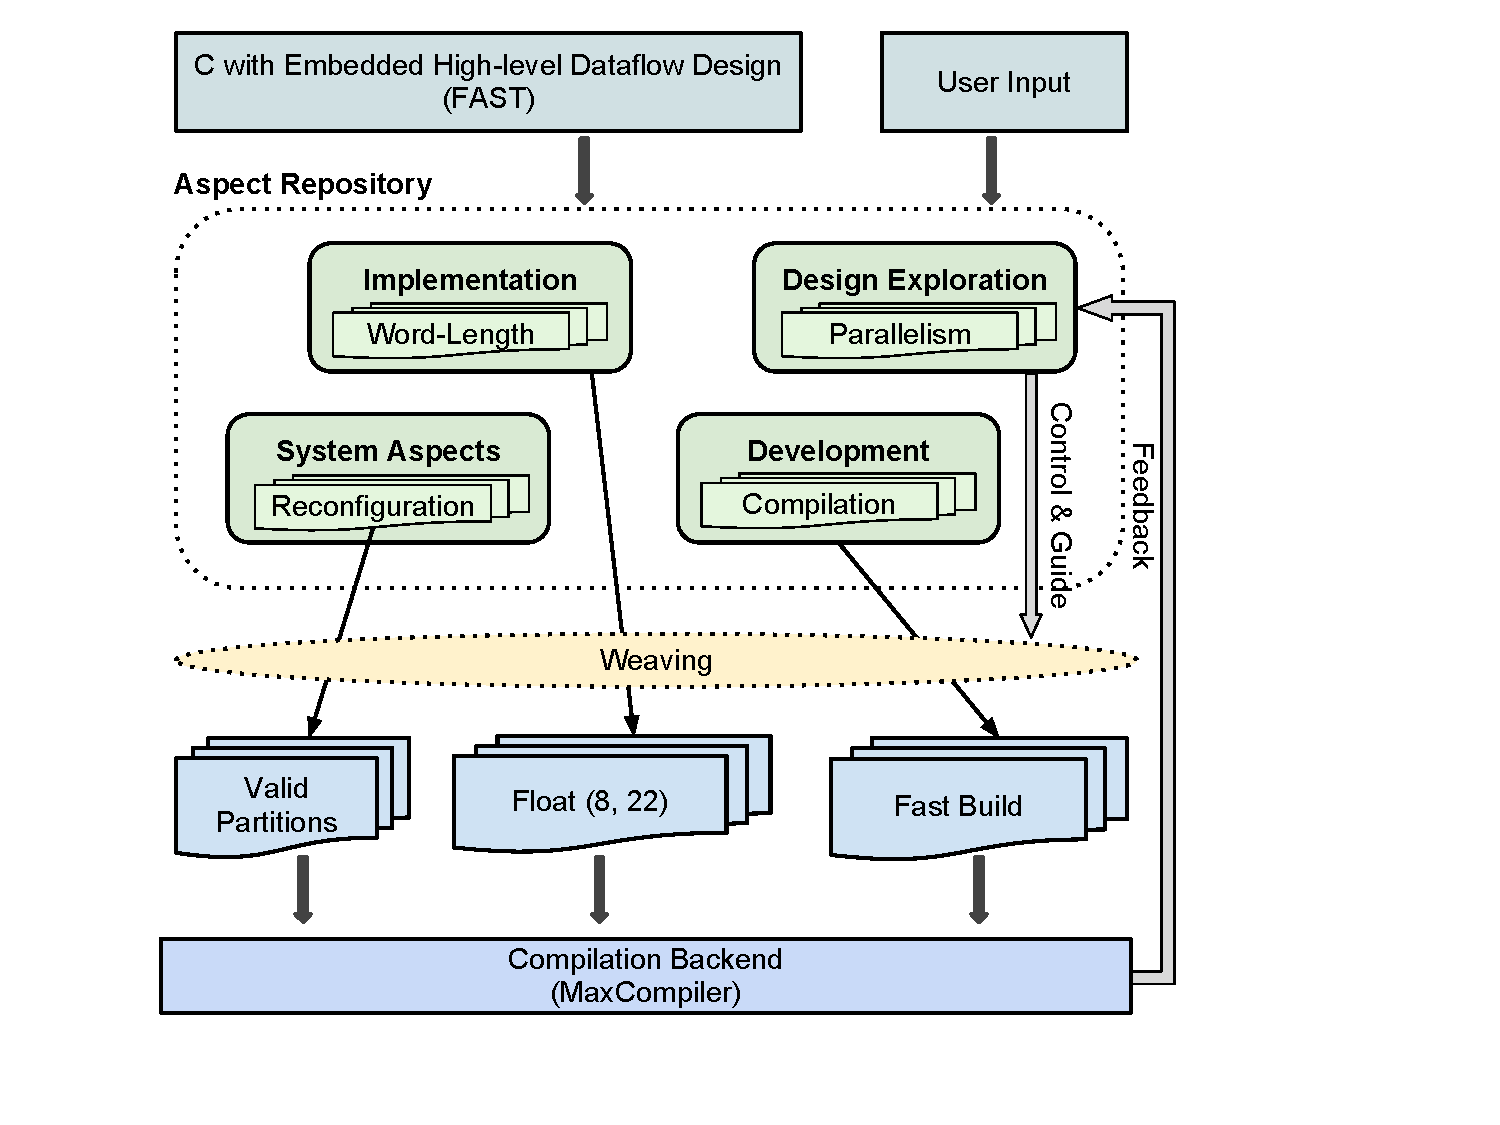
\includegraphics[scale=0.5, trim=60 50 0 0]{figs/design-flow}
  \caption{Proposed approach for aspect-driven compilation of dataflow
    designs.}
  \label{fig:design-flow-overview}
\end{figure}

The design flow produces as its output a number of implementations based on
requirements specified through aspects.

The following algorithm describes the operation of the proposed design flow:

\begin{lstlisting}
  for (in as do als)
\end{lstlisting}

\section{Design Goals}

Our design flow aims to improve both \emph{efficiency} (in terms of
performance and energy consumption) and \emph{productivity}. The
former is crucial to High Performance Computing, the latter helps
reduce development cost and time and is a well-known issue with
existing FPGA based acceleration solutions \XXX{cit. req.}. To achieve this we focus
on maintaining or improving the \emph{performance} and \emph{energy
  efficiency} of existing applications while using a more systematic
approach for design optimisation that results in more \emph{portable}
application code, improves \emph{integration} with existing
applications and \emph{automate} time consuming and error-prone tasks
that need to be performed manually using traditional tools.

\subsection{Performance}
To maintain performance of existing applications
\emph{Performance:} specify high-performance dataflow designs,
that achieve significant speedup over sequentially executed
implementations; exploit the reconfiguration capability of FPGA
devices to improve performance and efficiency;

\subsection{Energy Efficiency}

\subsection{Portability}
\emph{Portability:} improve portability of dataflow designs, to
allow reuse of optimisation strategies on various platforms;

\subsection{Integration}
\emph{Integration:} simplify translation of existing
applications to high-performance dataflow designs to facilitate the
integration of the proposed design flow with existing (predominantly
imperative) application code;

\subsection{Automation}
\emph{Productivity:} improve developer productivity by providing
high-level means of specifying dataflow designs and controlling
compilation strategies that reduce compilation time and generating
boilerplate code automatically.


\section{Steps}

To meet these requirements we propose the following approach.

Firstly, we introduce \FAST{} (described in Section \ref{sec:maxc}), a
novel language for specifying dataflow designs. We specify the
accelerated portion of the original applications using \FAST{}
dataflow kernels. By maintaining compatibility with C99 syntax we
improve developer productivity by providing a familiar language and
introduce the possibility of combining hardware and software
specifications. Secondly, by using an aspect driven compilation flow
we decouple optimisation from design development, improving design
portability, and we automate the generation of code and design space
exploration improving productivity. Finally, systematic design space
exploration is used to identify maximum performance configurations,
subject to platform specific constraints.

The proposed design flow is illustrated in Fig.~\ref{fig:design-flow}
and follows the steps:
\begin{enumerate}
\item a C application containing an embedded high-level dataflow
  design is developed from the original source application. The design
  is implemented using \FAST{} as described in Section~\ref{sec:maxc};
\item the dataflow design is transformed by the aspects in the
  repository to generate new designs (e.g. with multiple word-length
  configurations). The classes of aspects used with our approach are
  introduced in Section~\ref{sec:aspects};
\item the generated configurations are compiled using a backend
  compilation toolchain (currently MaxCompiler) to dataflow designs
  implemented on FPGAs;
\item the feedback from the compilation process is used to drive the
  design space exploration, repeating the weaving and compilation
  process until user specified requirements are met.
\end{enumerate}


\begin{figure}[!ht]
  \centering
  \def\svgwidth{\textwidth}
  \input{figs/asap13-design-flow.pdf_tex}
  \caption{Proposed approach for aspect-driven compilation of dataflow
   designs.}
  \label{fig:reconfig-design-flow}
\end{figure}

Compared to existing work described in
\cite{Cardoso:Teixeira:Alves:Nobre:Diniz:Cutinho:Luk:2012} and
\cite{cardoso2011new} our approach emphasises and provides more
freedom in the exploration of design level optimisation (such as word
length optimisations and mapping of arithmetic blocks to DSPs) by
using a combination of implementation aspects (shown in
Fig.~\ref{fig:design-flow}) and \FAST{} optimisation options.

Additionally, our approach targets a dataflow architecture as opposed
to the von Neumann architecture proposed in related work, which
typically includes a General-Purpose Processor (GPP) and a custom
accelerator. We consider additional optimisations to achieve
performance improvements as a result of a systematic design space
exploration process.

\section{Comparison with Existing Approaches}

\section{Extensions}

\subsection{Design Modelling}

\subsection{Run-time Reconfiguration Support}

Extensions to the original flow are required to support the automation
of run-time reconfiguration support. Figure
\ref{fig:reconfig-design-flow} presents an overview of the revised
design flow.

\begin{figure}[!ht]
  \centering
  \def\svgwidth{\textwidth}
  \input{figs/fpt13-design-flow.pdf_tex}
  \caption{Revised design flow to support run-time reconfiguration}
  \label{fig:reconfig-design-flow}
\end{figure}

\begin{enumerate}
\item From an initial C + FAST design we create a number of
  configurations by applying implementation and system aspects as
  described in ASAP.
\item For each configuration we derive a model of the resource usage,
  performance and power usage using modelling aspects (described in
  section 3)
\item Based on predicted models (from step 2) and possibly on existing
  empirical information from the Design DB we partition the
  application and schedule the partitions to achieve user requirements
  and optimization goals.
\item Finally a number of executables and designs are created,
  corresponding to the generated configurations from step 3. Based on
  compilation and execution (of automated performance tests) we refine
  our predictions for design resource usage, performance and power.
\end{enumerate}

Additionally the run-time environment has to be extended to support
this approach. An overview of the assumed runtime architecture for the
proposed approach is shown in Figure \ref{fig:reconfig-runtime}.

\begin{figure}[!ht]
  \centering
  \def\svgwidth{\textwidth}
  \input{figs/fpt13-runtime.pdf_tex}
  \caption{Run-time architecture required to support run-time reconfiguration}
  \label{fig:reconfig-runtime}
\end{figure}

\begin{enumerate}
\item The CPU drives the FPGA. It initiates the computation and
  monitors the FPGA for factors such as temperature and power.
\item The CPU can request the FPGA to abort execution of the current
  design. Current results are saved (i.e. streamed back to CPU)
  before reconfiguration is triggered.
\item The CPU can select a new design to be uploaded and
\item Empirical results are recorded in the Design Database, to
  improve future estimates of performance, power and thermal values.
\end{enumerate}

\section{Summary}
